% !TEX encoding = UTF-8 Unicode
\graphicspath{{figuras/}}

\chapter{Dicas do \LaTeX}
\label{cap2}

Dicas\footnote{Recomenda-se que todo capítulo seja iniciado com um parágrafo resumo introdutório do capítulo descrevendo o assunto e o escopo ou principais tópicos abordados.} de uso e exemplos de recursos do \LaTeX \, são apresentados. O \LaTeX\,   é uma ferramenta poderosa para editar relatórios técnicos pois nos permite estruturar o conteúdo com citações e referências cruzadas para figuras, código de programa e equações de forma programática. Acrescentar ou modificar textos no \LaTeX\, é facilitado, pois figuras e listagens de códigos podem ser armazenadas em arquivos externos e incluídos facilmente no corpo do texto. As modificações feitas nas figuras ou códigos são automaticamente formatadas. Além disso, a ideia central do \LaTeX, \, que é baseada em macros, nos permite personalizar trechos de texto que se repetem ou que desejamos que possuam um comportamento predefinido. Divirta-se!

\section{Algumas dicas ilustrando  recursos do \LaTeX}

As dicas a seguir ajudam não apenas a editar um texto \LaTeX\, com uma sintaxe mais limpa, mas também a editar equações, mencionar corretamente citações e organizar a inserção de figuras isoladas ou agrupadas, com ou sem legenda para o grupo.  A inclusão de listagens de códigos de programas também é usual e recomenda-se o uso do pacote \verb|mcode| já corrigido para usar caracteres acentuados em comentários de programas fonte.

De início, destacamos a parte mais importante de um texto técnico: mencionar os créditos a quem publicou anteriormente trabalhos técnicos que usamos diretamente no trabalho que descrevemos. A diferença entre plágio e pesquisa é exatamente sobre isso. Pesquisa e desenvolvimento são realizados  buscando em diversas fontes  informações, procedimentos, algoritmos, etc., \textbf{citando a fonte com clareza} e onde é  obtida. \textbf{Plágio} é aquilo que se copia de um único trabalho ou de alguns poucos, mas as referências são omitidas para se ocultar os verdadeiros autores. Plágio é crime além de ser uma vergonha acadêmica e profissional que causa desonra e cerceamento explícito dos pares (colegas de profissão, de sociedades técnico-científicas, etc.).

Recomenda-se o uso do aplicativo \cite{JabRef2021} para editar e organizar bancos de dados com as referências bibliográficas. O arquivo \verb|MinhasReferencias.bib| contém uma lista de referências usadas neste documento como exemplo.

\paragraph{Citações} de referências bibliográficas fazem parte da essência do \LaTeX. Para citar um livro, e.g. vou citar um livro clássico mas difícil de ler e entender que é \cite{Astrom:1970}. O código para inserir esta referência cruzada é: \verb|\cite{Astrom:1970}|.  Um livro também clássico e muito bom é \cite{Astrom:1997}. O livro considerado a bíblia da Eletrônica é \cite{Horowitz:1981307}, que é referenciado usando o código: \verb|\cite{Horowitz:1981307}|. Todas estas referências estão na pasta junto deste gabarito no arquivo texto \mcode{ref_books.bib}.

Notas de aula podem ser citadas se forem usadas como referência no desenvolvimento de suas atividades e.g \cite{BragaAR2019} e citações para este documento que é um gabarito de relatório técnico com algumas dicas \LaTeX \cite{bragaAR2021} (\verb| \cite{bragaAR2021}|).

\subsection{Figuras}

Figuras são importantes não apenas para ilustrar  graficamente algum local, conceito ou procedimento, mas porque o ditado popular, \emph{uma imagem vale mais que mil palavras}, é realmente impactante e precisa ser bem realizado. 
Para se editar figuras existem diversos aplicativos. Recomenda-se ao interessado  explorar as virtudes e potencialidades dos pacotes do Latex TikZ (\cite{pgftikz}) e  Circuitikz (\cite{circuitikz}). Desenhar programando é dificil no início até se acostumar oom a sinttaxe e os conceitos porém, depois de dominados os comandos, é uma elegância obtida apenas por profissionais.


Figuras são referenciadas com o rótulo {\textit{Figura}} seguido do caracter \verb|~| (\emph{nonbreaking space}) e de uma referência numérica \textit{sem parênteses}, e.g. 

A linha a seguir:

\begin{verbatim}
 O Diagrama de Blocos mostrado na  Figura~\ref{fig:cap1_MBPC_blk_diag} 
 ilustra  uma arquitetura (...)
\end{verbatim}

resulta no seguinte texto formatado:

\fbox{O Diagrama de Blocos mostrado na  Figura~\ref{fig:cap1_MBPC_blk_diag} ilustra uma arquitetura(...)}

Para facilitar a edição de referências às figuras definiu-se a macro  \verb|\figref|. Desta forma podemos alterar globalmente as referências às figuras modificando a macro   \verb|\newcommand\figref{fig.~\ref}| no caso de se desejar economizar espaço como em formatação de artigos.

	A inserção de figuras é facilitada pelo pacote \verb|\usepackage{keyfloat}|. Além de simplificar a sintaxe, o pacote \verb|keyfloat| provê parâmetros e ambientes para agrupar figuras, tabelas e textos arranjados matricialmente\footnote{O pacote \emph{keyfloat} tem sido atualizado enquanto que os pacotes \emph{subfig} e \emph{subfigure} já são considerados obsoletos pela incompatibilidade com hyperlinks em arquivos $*.pdf$.}. O  modo tradicional de inserir figuras, e.g.
	
	
\begin{keyfigure}{c= {Sintaxe clássica para inserir uma figura.},l=lst:IncludeFigura}
\lstset{language=[Latex]Tex}
\begin{highlightblock}
\begin{figure}[!htbp]
	\centering
	\includegraphics[width=15cm]{cap1_MBPC_blk_diag} 
	\caption{Arquitetura simplificada de um sistema de controle baseado em 
		modelo 	com a função de Auditor de Processo. Se desejar inserir 
		referência cruzada na legenda, lembre-se de proteger o comando com 
		\emph{protect}: Uma figura que se liga a uma bela 
		equação \protect\bref{eq:piuBella}.}
	\label{fig:cap1_MBPC_blk_diag}
\end{figure}
\end{highlightblock}
\end{keyfigure}

Os parâmetros \verb|[!htbp]| indicam a sequência de prioridade para posicionar a figura: \textsf{h} here (aqui!), \textsf{t} top (no topo da página), \textsf{b} bottom (na parte inferior da página) e \textsf{p} page (numa página só de figuras).
%--- inseção de figura usando includegraphics{}--------
\begin{figure}[!htbp]
	\centering
	\includegraphics[width=15cm]{cap1_MBPC_blk_diag} 
	\caption{Arquitetura simplificada de um sistema de controle baseado em modelo com a função de Auditor de Processo. Se desejar inserir referência cruzada na legenda, lembre-se de proteger o comando com \emph{protect}: Uma figura que se liga a uma bela equação \protect\bref{eq:piuBella}.}
	\label{fig:cap1_MBPC_blk_diag}
\end{figure}
% ---------------------------------------------------------

No pacote \verb|keyfloat| as figuras são organizadas ou  arranjadas  usando  o ambiente \verb|keyfloats| como descrito no código \ref{lst:FigKeyfloat1} cujo resultado está ilustrado nas Figuras~\ref{fig:SubFloatA}, \ref{fig:SubFloatB}, \ref{fig:SubFloatC} e na Tabela~\ref{tab:SubFloatD}.  Note bem, este arranjo de figuras com uma tabela inserida como a Tabela~\ref{tab:SubFloatD} é horroso. Isso foi feito apenas para ilustrar uma das várias possibilidades de arranjo de figuras e tabelas.

\begin{keyfigure} {c= {Sintaxe \emph{keyfloats} para inserir um grupo de figuras sem legenda para a figura toda.},l=lst:FigKeyfloat1}
\lstset{language=[Latex]Tex}
\begin{highlightblock}
	\begin{keyfloats}{3}[lw=1,h=15em,kar,va=c]
		\keyfig{lw=1,f,c={Primeira subfigura: A},	l=fig:SubFloatA,
			t={\textsf{Texto opcional.}} }{example-image-a}
		\keyfig{lw=1,f,r=90,c={Segunda subfigura: B},l=fig:SubFloatB, 
			t={\textsf{Texto opcional.}} }{example-image-b}
		\begin{keyfloats}{1}[lw=1,kar]
			\keyfig{lw=1,f,c={Terceira subfigura: C},
							l=fig:SubFloatC}{example-image-c}
			\keytab{c={Uma tabela incluída como Quarta subfigura: D},
				l=tab:SubFloatD}{% --- Inicio Tabela
				\begin{tabular}{l l} 
					\hline Item & Descrição\\ \hline
					1 & Letra A \\
					2 & Letra B \\
					\hline
				\end{tabular}%
			}% --- fim tabela
		\end{keyfloats}
	\end{keyfloats}
\end{highlightblock}
\end{keyfigure}
Os parâmetros ou \emph{key=values} usuais do \verb|\begin{keyfloats}{1}[lw=1,h=15em,kar,va=c]| são:
	\begin{itemize}
		\item \textbf{c={legenda}} parâmetro com a legenda entre chaves, e.g. c={Minha legenda, com vírgula tem que ser delimitada por chaves.}.
		\item \textbf{l=label}  tag ou rótulo, e.g. l=fig:Minhafigura.
		\item \textbf{lw=1} ajusta a largura da figura para o \emph{line width} da célula da subfigura.
		\item \textbf{h=15em} ajusta a altura da figura, que neste exempo é igual 15em (altura do caracter M).
		\item \textbf{va=c} alinha as figuras verticalmente no centro, c=center (default). Pode ser variado para b=base, t=topo.
		\item \textbf{kar} \emph{kar = Keep AspectRatio} da subfigura.
		\item \textbf{s=0.5} ajusta manulamente a escala da figura para a metade do tamanho.
	\end{itemize}
	
	O ambiente \verb|keyfloats| pode ser aninhado e o parâmetro  do ambiente \verb|\begin{keyfloats}{3}| especifica 3 colunas, sendo a subfigura 4 e a tabela 1 agrupados em uma mesma coluna com o ambiente aninhado  \verb|\begin{keyfloats}{1}| .
			
			%--- inseção de figuras usando arranjo de floats.
			\begin{keyfloats}{3}[lw=1,h=15em,kar,va=c]
				\keyfig{lw=1,f,c={Primeira subfigura: A},	l=fig:SubFloatA,
					t={\textsf{Texto opcional.}} }{example-image-a}
				\keyfig{lw=1,f,r=90,c={Segunda subfigura: B},l=fig:SubFloatB, 
					t={\textsf{Texto opcional.}} }{example-image-b}
				\begin{keyfloats}{1}[lw=1,kar]
					\keyfig{lw=1,f,c={Terceira subfigura: C},l=fig:SubFloatC}{example-image-c}
					\keytab{c={Uma tabela incluída como Quarta subfigura: D},l=tab:SubFloatD}{% --- Inicio Tabela
						\begin{tabular}{l l} 
							\hline Item & Descrição\\ \hline
							1 & Letra A \\
							2 & Letra B \\
							\hline
						\end{tabular}%
					}% --- fim tabela
				\end{keyfloats}
			\end{keyfloats}
			% ---------------------------------------------------------
			
			
			O ambiente \verb|keysubfigs| é recomendado quando  as subfiguras fazem parte de uma figura com legenda para o conjunto de subfiguras (vide Figura~\ref{fig:LabelAll}) e que contém legendas para suas subfiguras \subref{fig:SubfigA},  \subref{fig:SubfigB},  \subref{fig:SubfigC} e  \subref{fig:SubfigD}. Cada subfigura é referenciada diretamente usando \emph{label} completo (\verb|\ref{fig:SubfigA}| $\rightarrow$ \ref{fig:SubfigA}) ou apenas a referência interna na figura (\verb|\subref{fig:SubfigA}| $\rightarrow$  \subref{fig:SubfigA}). 
			
			O ambiente \verb|keysubfigs| requer além do parâmetro designando o número de colunas, uma lista de parâmetros estabelecendo a legenda e o \emph{label} como segue:

\begin{keyfigure}{c= {Sintaxe \emph{keysubfigs} para inserir uma figura com uma legenda para a figura toda.},l=lst:FigKeysubfig}
	
\begin{highlightblock}
\lstset{language=[Latex]Tex}
\begin{keysubfigs}{3}{c={Legenda da figura toda.},l=fig:LabelAll}
	\keyfig{lw=1,f,c={Subfigura A},	l=fig:SubfigA,
		t=Explicando esta figura!}{example-image-a}
	\keyfig{lw=1,f,r=90,c={Subfigura B},
		l=fig:SubfigB, 	t= Uma explicação bem longa desta figura é formatada 
		dentro dos limites da figura!.}{example-image-a}
	\begin{keyfloats}{1}
		\keyfig{lw=1,f,c={Subfigura C},l=fig:SubfiguraC}{example-image-a}
		\keytab{c={Subfigura D},l=fig:SubfigD} 
		{Uma matriz: $A = \mqty[1 & 2 \\ 3 & 4]$}
	\end{keyfloats}
\end{keysubfigs}

\end{highlightblock}

\end{keyfigure}


%%%%%%%
\begin{keysubfigs}{3}{c={Legenda da figura toda.},l=fig:LabelAll}
	\keyfig{lw=1,f,c={Subfigura A},	l=fig:SubfigA,
				t=Explicando esta figura!}{example-image-a}
	\keyfig{lw=1,f,r=90,c={Subfigura B},
		l=fig:SubfigB, 	t= Uma explicação bem longa desta figura é formatada 
		dentro dos limites da figura!.}{example-image-a}
	\begin{keyfloats}{1}
		\keyfig{lw=1,f,c={Subfigura C},l=fig:SubfigC}{example-image-a}
		\keytab{c={Subfigura D},l=fig:SubfigD}{Uma matriz: $A = \mqty[1 & 2 \\ 3 & 4]$}
	\end{keyfloats}
\end{keysubfigs}


Para inserir códigos de programa, recomendamos usar o ambiente \mcode{lstlisting} que é importado pelo pacote \mcode{mcode}. O arquivo \mcode{mcode.sty} já contém uma correção para comentários em  português. O pacote \mcode{lstlistings} não imprime comentários com caracteres acentuados corretamente!
Observe que o pacote \mcode{mcode.sty} insere códigos fonte de programas (vide Programa~\ref{lst:codigoFigura}) mantendo a endentação ou recuo de texto correto.

% --- Inserindo código Matlab
\lstset{language=Matlab} % selecionando a linguagem para formatação
\begin{lstlisting}[numbers =none, caption= {Sintaxe Matlab.}, label=lst:FigKeymat]
	R = 221e3
	C = 47e-9 %
	%C = 470e-12
	f_c = 1/(2*pi*R*C) % frequencia de corte do filtro
	num2eng(f_c,4) % Frequencia de corte do filtro
	if x>1, x=3; 
	end
\end{lstlisting}

O código fonte Latex para inserir uma figura com legenda e rótulo de referência está ilustrado no Programa~\ref{lst:codigoFigura}.

\begin{keyfigure}{ c= {Inserindo código fonte \LaTeX\, usando o ambiente  \texttt{highlightblock}  lstlisting.},l=lst:codigoFigura}
	\lstset{language=[Latex]Tex}
	\begin{highlightblock}
		\begin{figure}
			% insercao de arquivo ou codigo Tikz de figura
			\includegraphics{figuras/cap1_MBPC_blk_diag} 
			%-----------------------------------------------
			\caption{Uma legenda}  %O caption tem que preceder o label!
			\label{fig:cap1mbpcblkdiag}
		\end{figure}
	\end{highlightblock}
\end{keyfigure}

Inserindo código fonte \LaTeX\, usando o ambiente  \texttt{highlightblock}\footnote{O ambiente \texttt{highlightblock} substitui o ambiente clássico do \texttt{Verbatim}} resulta em:

\lstset{language=[Latex]Tex}
\begin{highlightblock}
	\begin{figure}
		% inserção de arquivo ou codigo Tikz de figura
		\includegraphics{figuras/cap1_MBPC_blk_diag} 
		%---------------------------------------------------
		\caption{Uma legenda}  %O caption tem que preceder o label!
		\label{fig:cap1mbpcblkdiag}
	\end{figure}
\end{highlightblock}

Um exemplo de diagrama esquemático desenhado usando o pacote Tikz e Circuitikz está ilustrado na Figura~\ref{fig:diagEsquematico}. O código fonte CircuiTikZ usado nesse exemplo está listado no Programa~\ref{code:ExemploTikz}.

\begin{keyfigure}{lw=0.5,kar,
	c={Diagrama esquemático. O código Latex está listado no Programa~\protect\ref{code:ExemploTikz}.},
	l=fig:diagEsquematico
}
%%------------------------------------------------------------------- %%
%  fig:ExemploCircuiTikz
% Diagrama em esquemático de um  filtro  analógico RC
%
%  --- Anisio R. Braga, COLTEC-UFMG
%  --- 2021/01/25
%---------------------------------------------------------------------
%--- Template
\tikzset{blockdef/.style={% bloque
		{Straight Barb[harpoon, reversed, right, length=0.2cm]}-{Straight Barb[harpoon, 
			reversed, left, length=0.2cm]},blue!50!gray}} 
%------------------------------------------------------------
\scalebox{1}{% Envelope para redimensionar
	\begin{circuitikz}[scale=1, transform shape, cute inductors]
		\ctikzset{resistors/scale=0.7,  capacitors/scale=0.7, inductors/scale=0.8,diodes/scale=0.5}
		\ctikzset{american open voltage=legacy}
		\tikzstyle{bkgbox}=[draw, rectangle, inner sep=25pt, densely dotted, rounded corners=1mm, 
		teal, color=teal!50!gray,thick, fill=teal!5]
		% --- Gridlines
		\def\Xgrid{7}   	\def\Ygrid{5} 
		%	\draw[step=2mm] [help lines, black!10]  (-\Xgrid,-\Ygrid) grid (\Xgrid,\Ygrid);
		%	\draw[step=10mm] [help lines, blue!30]  (-\Xgrid,-\Ygrid) grid (\Xgrid,\Ygrid);
		%	\foreach \x in {-\Xgrid, ...,\Xgrid} \node at (\x,-\Ygrid) [below,font=\scriptsize] {\x}; 
		%	\foreach \x in {-\Xgrid, ...,\Xgrid} \node at (\x,\Ygrid) [above,font=\scriptsize] {\x}; 
		%	\foreach \y in {-\Ygrid, ...,\Ygrid} \node at (-\Xgrid,\y) [left,font=\scriptsize] {\y}; 
		%	\foreach \y in {-\Ygrid, ...,\Ygrid} \node at (\Xgrid,\y) [right,font=\scriptsize] {\y}; 
		\node at (0,4)[align=center, font=\large] {CircuiTikZ's Template};
		
		% --- Definitions -----------
		\def\dx{2}	\def\dy{2}
		%---------------------------
		
		%--- Circuito interno
		\draw[]  (0,0) \coord(a2) to[open] ++(0,\dy)\coord(a1)
		(a1)   to[R, l=$R$] ++(\dx,0)\coord(b1)
		(b1)   to[C, l_=$C$,-*] ++(0,-\dy)\coord(b2)
		(b2)   to[short] (a2);
		
		\node at (b2) [ground, label={[shift={(0.5,-0.5)}] \SI{0}{\volt} }] {};
		%--- Terminais
		\draw[]    (a1)   to[short,-o] ++(-0.75*\dx,0)\coord(a11)
		(a2)   to[short,-o] ++(-0.75*\dx,0)\coord(a21);
		
		\draw[]    (b1)   to[short,*-o] ++(0.75*\dx,0)\coord(b11)
		(b2)   to[short,-o] ++(0.75*\dx,0)\coord(b21);
		
		% --- Correntes
		\draw[icolor, color=icolor]    (a11)   to[open,f =$i$] (a1);
		% --- Probes
		\probe[azul]{a11}[-180:0.35]{A}[$1$]
		\probe[black]{a21}[-180:0.35]{Ci}[$-$]
		
		\probe[laranja]{b11}[0:0.35]{B}[$2$]
		\probe[black]{b21}[0:0.35]{Co}[$-$]
		% --- Voltímetros
		\draw[european, icolor, color=icolor] (A) to[open, v=$V_{1}$,voltage/european label distance =-1.75] (Ci);
		\draw[european, vcolor, color=vcolor] (B) to[open, v^=$V_{2}$,voltage/european label distance =-1.75] (Co);
		% --- bloque
		\draw [blockdef] ($(a2)+(-1,-1.25)$) -- node[midway, fill=white,align=center,font=\scriptsize]{Filtro\\ Passa-Baixas} ($(b2)+(1,-1.25)$);
		% --- Destacando blocos de circuito no background
		\begin{pgfonlayer}{background}       
			\node[fit=(a2) (a1)  (b1) (b2),bkgbox, gray, fill=teal!5]{};
		\end{pgfonlayer}
		%-------------------------------------------------
	\end{circuitikz}
}% fim do scalebox
 % insere figura Tikz sem escalonar
\end{keyfigure}

\lstinputlisting[label={code:ExemploTikz},caption={Exemplo de código para desenhar circuitos  usando o CircuiTikZ}, basicstyle=\tiny ] {figuras/ExemploCircuitikz.tikz}

Quando usar referência cruzada na legenda de figuras recomenda-se proteger o comando \mcode{ref} ou \mcode{cite} acrescentando o prefixo \mcode{protect} como ilustra a sintaxe a seguir:
\begin{verbatim}
\protect\ref{lst:codigoFigura}
\protect\cite{Astrom:1970}
\end{verbatim}


\subsection{Equações} 
Para editar equações inseridas numa linha de texto como esta: $ E = m\cdot c^2 $ insira a equação entre dois  caracteres \$, e.g.
\begin{verbatim}
	$ E = m\cdot c^2 $ 
\end{verbatim} 

Para editar equações que se deseja referenciar no texto use o ambiente \mcode{equation} com um rótulo (\mcode{label}) como segue:

\begin{verbatim}
	\begin{equation} \label{eq:piuBella}
		\frac{dy}{dt} = a y.   
	\end{equation}
\end{verbatim}
A referência a uma equação é feita usando numeração entre parênteses, e.g. a equação \bref{eq:piuBella} é uma das mais belas equações matemáticas.

\begin{equation} \label{eq:piuBella}
	\frac{dy}{dt} = a y.   
\end{equation}

Uma forma mais elegante de editar equações é usando o pacote \emph{physics} que resulta em uma equação com o operador derivada: \verb|$\dv{y}{t}$| para formatar $\dv{y}{t} = a \, y$ ou simplesmente   \verb|$\dd{t}$| para formatar $\dd{t}$, representado com fonte \emph{roman} e não itálico. Os exemplos a seguir ilustram o uso destes operadores. 
\begin{align} \label{eq:piuBella2}
	\dv{y}{t} &= a \, y, \\  % note o uso do comando \, para inserir um pequeno espaço entre a e y.
	y &= \int \dv{y}{t} \dd{t}.   % note o uso do comando \, para inserir um pequeno espaço entre a e y.
\end{align}
Ao escrever a função exponencial lembre-se de escrever a constante $\text{e}=2.71828\cdots$ usando o formato de texto, \verb|$\text{e}^{-t/\tau}$| que produz: $\text{e}^{-t/\tau}$.


Para inserir matrizes  uma codificação é como segue:
\begin{verbatim}
	$D = \begin{bmatrix} 
		1   &  0 &    0\\
		-1   &  1&     0\\
		0   & -1 &    1
	\end{bmatrix}$, 
	%você pode escrever tudo em uma linha pois a quebra de linha é feita porr "\\"
	$ S = \begin{bmatrix} 1    & 0   &  0\\ 1    & 1   &  0\\ 1   &  1   &  1 \end{bmatrix}$,
	$x = \begin{bmatrix} 3\\ 1\\ 9 \end{bmatrix}$,   
	$Dx = \begin{bmatrix} 3\\ -2\\8 \end{bmatrix}$, 
	$Sx = \begin{bmatrix} 3\\ 4\\ 13 \end{bmatrix}$
\end{verbatim}

que resulta em

$D = \begin{bmatrix} 
	1   &  0 &    0\\
	-1   &  1&     0\\
	0   & -1 &    1
\end{bmatrix}$, 
%você pode escrever tudo em um linha lembrando de usar a quebra de linha no modo matemático "\\"
$ S = \begin{bmatrix} 1    & 0   &  0\\ 1    & 1   &  0\\ 1   &  1   &  1 \end{bmatrix}$,
$x = \begin{bmatrix} 3\\ 1\\ 9 \end{bmatrix}$,   $Dx = \begin{bmatrix} 3\\ -2\\8 \end{bmatrix}$, $Sx = \begin{bmatrix} 3\\ 4\\ 13 \end{bmatrix}$

Todavia, usando o pacote \mcode{physics} fica mais  fácil e limpo a codificação:
\begin{verbatim}
	$D = \bmqty{1   &  0 &    0\\-1   &  1&     0\\0   & -1 &    1}$, 
	$ S = \bmqty{ 1    & 0   &  0\\ 1    & 1   &  0\\ 1   &  1   &  1 }$, 
	$x = \bmqty{ 3\\ 1\\ 9 }$,   
	$Dx = \bmqty{ 3 \\ -2 \\ 8 }$, 
	$Sx = \bmqty{ 3\\ 4\\ 13 }$.
\end{verbatim}

que resulta em 
$D = \bmqty{1   &  0 &    0\\-1   &  1&     0\\0   & -1 &    1}$, $ S = \bmqty{ 1    & 0   &  0\\ 1    & 1   &  0\\ 1   &  1   &  1 }$, $x = \bmqty{ 3\\ 1\\ 9 }$,   $Dx = \bmqty{ 3 \\ -2 \\ 8 }$, $Sx = \bmqty{ 3\\ 4\\ 13 }$.


Se quiser apresentar uma matriz de forma adensada, o pacote \mcode{physics} tem o comando 
\begin{verbatim}
	$ S = \sbmqty{ a  & b  \\ c  & d   }$
\end{verbatim}
que resulta em $ S = \sbmqty{ a  & b  \\ c  & d   }$.

O pacote \mcode{physics} também cria uma sintaxe elegante para digitar funções como seno e cosseno.
A equação $\sin[2](\theta) + \cos[2](\theta)=1$ é digitada usando o pacote \mcode{physics} como
\begin{verbatim}
	$\sin[2](\theta) + \cos[2](\theta)=1$.
\end{verbatim}

Para entender os recursos do pacote \mcode{physics}, leia o manual \mcode{https://ctan.org/pkg/physics?lang=en}.


Para citar termos em verbatim use o ambiente \mcode{mcode} do pacote \mcode{mcode.sty}. Aliás, este pacote \mcode{mcode.sty} já contém as correções para comentários com caracteres acentuados como os do português.

Uma equação é facilmente editada com índices:
\begin{verbatim}
	\begin{equation}\label{eq:QuedaVoltagem}
		v_{AB} = v_A - v_B. 
	\end{equation}
\end{verbatim}

que processado pelo \LaTeX \, resulta em
\begin{equation}\label{eq:QuedaVoltagem}
	v_{AB} = v_A - v_B. 
\end{equation}

Para escrever  somatórios e potência de variáveis usamos como exemplo a expressão de desvio padrão: 
\begin{verbatim}
	\begin{equation} \label{eq:desvioPadrao}
		s_x =\sqrt{\frac{1}{N-1}\sum_{k=1}^{N} \qty(x_k - \bar{x})^2},
	\end{equation}
\end{verbatim}

Que resulta em:
\begin{equation}\label{eq:desvioPadrao}
	s_x =\sqrt{\frac{1}{N-1}\sum_{k=1}^{N} \qty(x_k - \bar{x})^2},
\end{equation}
em que $\bar{x}$ representa a média dos valores $x_k$. Observe como se pontua uma equação com vírgula \bref{eq:desvioPadrao} e ponto final \bref{eq:QuedaVoltagem}. Note o uso do comando \mcode{bref\{\}} para referenciar equações. O comando \mcode{bref\{\}}  está definido no preâmbulo do masterdoc como
\begin{verbatim}
	\newcommand{\bref}[1]{\mbox{(\ref{#1})}}
\end{verbatim}
é simplesmente  uma macro usada para facilitar referência às equações sem esquecer de envolver o número de referência entre parêntesis. 


\subsection{Edição e formatação de Sistemas de Unidades}

O uso correto das unidades de medida é muito importante em aplicações e publicações técnicas. O Système International d'Unités (SI)  estabeleceu definições para um sistema de unidades coerente que é globalmente aceito como padrão.  O SI estabeleceu convenções tipográficas para a exibição correta de números e unidades  para minimizar ambiguidades e garantir uma representação correta do significado de unidades em publicações.
O pacote \emph{siunitx}  fornece um método unificado para usuários LATEX para escrever números e unidades de forma correta e fácil. A filosofia de design do pacote \emph{siunitx} permite que as regras do SI sejam  configuradas com opções  flexíveis para atender aos requisitos variados de editores, autores, universidades, etc., sem a necessidade de alterar a edição com as macros  do \emph{siunitix}. Embora a edição com as macros do \emph{siunitix} pareça demasiadamente verbosa e extensa, o uso destas macros  assegura coerência e facilita a compreensão do significado literal das unidades. 

A Tabela~\ref{tab:siunitx} ilustra o uso de algumas macros do \emph{siunitx} e respectivas formatações. 

Ao fazermos análise dimensional de alguma expressão matemática com unidades é frequente  o cancelamento de unidades que com o pacote \emph{SIunitx}  é facilitado com a seguinte sintaxe:

\verb|\unit[per-mode = fraction] {\cancel\kilogram\metre\per\cancel\kilogram\per\second} | 

que é formatada como  \unit[per-mode = fraction] {\cancel\kilogram\metre\per\cancel\kilogram\per\second}. Note que a macro do SIunitx  formata corretamente unidades com fonte romana não itálica e os espaços entre as unidades.

\keytab[H]{lw=1, c={Exemplos da sintaxe do \emph{SIunitx}.}, l=tab:siunitx}{
		\begin{tabu*}{l l} 
		\toprule {SIunitx} & {Formatação} \\ \midrule 
		\verb|$R_1 = \SI{2.7}{\mega\ohm}$| & $R_1 = \SI{2.7}{\mega\ohm}$\\ 
		\verb|$R_2 = \SI{10}{\kilo\ohm}$| & $R_2 = \SI{10}{\kilo\ohm}$\\ 
		\verb|$L_1 = \SI{1.59}{\nano\henry}$| & $L_1 = \SI{1.59}{\nano\henry}$\\ 
		\verb|$V_{12} = \SI{3.16}{\micro\volt}$| & $V_{12} = \SI{3.16}{\micro\volt}$\\ 
		\verb|$C_s =\SI[per-mode=symbol]{0.1}{\micro\farad\per\meter}$| & $C_s =\SI[per-mode=symbol]{0.1}{\micro\farad\per\meter}$ \\ 
		\verb|\si[per-mode=symbol]{\pico\farad\per\meter}| & \si[per-mode=symbol]{\pico\farad\per\meter} \\ 
		\verb|\unit{kg.m.s^{-1}}| & \unit{kg.m.s^{-1}}  \\ 
		\verb|\unit{\kilogram\metre\per\second}| & $\unit{\kilogram\metre\per\second}$ \\ 
		{\small \verb|\unit[per-mode=symbol]{\kilogram\metre\per\second}|}& \unit[per-mode = symbol]
		{\kilogram\metre\per\second} \\ 
		\verb|\num{2.7e-3}| & \num{2.7e-3} \\ 
		\verb|$\phi = \ang{45}$| &$\phi = \ang{45}$\\ 
	 \bottomrule 
	\end{tabu*} 
}


\section{Comentários finais}

Foram apresentadas  dicas básicas do \LaTeX\, exemplificadas com códigos fontes e respectivos pacotes usados. Os rótulos de seções, equações e figuras do \LaTeX\, foram ilustrados  no encadeamento de ideias por meio de referências cruzadas alinhavando os elementos referenciados no texto não apenas internamente no capítulo, mas também com todas as demais partes do relatório técnico\footnote{A conclusão de um capítulo consiste num breve resumo das ideias e assuntos abordados para relembrar o leitor o que foi explanado e com que relevância. Os comentários finais estabelecem uma transição suave encadeando logicamente os capítulos.}.